% !TeX root = bare_conf.tex
\documentclass[10pt, conference, a4paper]{IEEEtran}
\usepackage{amsmath,amsxtra,amssymb,amsthm,latexsym,amscd,amsfonts}
\usepackage[utf8]{vietnam}
\usepackage[top=2.7cm, bottom=5.4cm, left=2.72cm, right=3.0cm]{geometry}
\headsep=0.7cm
\headheight=1.0cm
\footskip=1.0cm
\voffset=-0.74cm

\usepackage{fancyhdr}
\pagestyle{fancy}
\renewcommand{\sectionmark}[1]{\markright{\MakeUppercase{#1}}{}}
\renewcommand{\headrulewidth}{0pt}

\ifCLASSINFOpdf
\usepackage[pdftex]{graphicx}
\usepackage{tikz}
\usepackage{pgfplots}
\pgfplotsset{compat=1.17}
\DeclareGraphicsExtensions{.pdf,.jpeg,.png,.jpg}
\else
\usepackage[dvips]{graphicx}
\DeclareGraphicsExtensions{.eps}
\fi

\usepackage{array}
\usepackage{url}
\usepackage{ragged2e}
\usepackage{float}
\usepackage[caption=false,font=footnotesize]{subfig}
\usetikzlibrary{arrows.meta,positioning,shapes.geometric,shapes.misc}

\newcolumntype{L}[1]{>{\RaggedRight\arraybackslash}p{#1}}
\setlength{\emergencystretch}{2em}

\makeatletter
\def\ps@IEEEtitlepagestyle{%
\def\@oddhead{\centering{\mbox{\footnotesize{\textit{\;\;\;\; Bài tập lớn: Môn Phát triển phần mềm mã nguồn mở -- Đại học Sài Gòn, 25/04/2026}}}}%
\def\@evenhead{\centering{\mbox{\footnotesize{\textit{\;\;\;\; Bài tập lớn: Môn Phát triển phần mềm mã nguồn mở -- Đại học Sài Gòn, 25/04/2026}}}}}%
\def\@oddfoot{\scriptsize \thepage \hfil }%
\def\@evenfoot{\scriptsize \hfil \thepage}
}
}
\makeatother

\begin{document}
\pagenumbering{arabic}
\fontsize{10}{12}
\selectfont

\fancyhead[C]{\footnotesize\textit{Bài tập lớn: Môn Phát triển phần mềm mã nguồn mở -- Đại học Sài Gòn, 25/04/2026}}

\title{\Large SmartDoc AI - Intelligent Document Q\&A System}

\author{\IEEEauthorblockN{Huỳnh Thanh Bình\IEEEauthorrefmark{1}, Lê Thanh Bình\IEEEauthorrefmark{2}, Trần Quốc An\IEEEauthorrefmark{3}}
	\IEEEauthorblockA{\IEEEauthorrefmark{1}Khoa Công nghệ Thông tin, Trường Đại học Sài Gòn, \IEEEauthorrefmark{2}Khoa Công nghệ Thông tin, Trường Đại học Sài Gòn,}
	\IEEEauthorblockA{ \IEEEauthorrefmark{3}Khoa Công nghệ Thông tin, Trường Đại học Sài Gòn}
	\IEEEauthorblockA{Email: thanhbinhitsgu17@gmail.com; binhle.230204@gmail.com;}
	\IEEEauthorblockA{quocan529@gmail.com}
}

\maketitle

\begin{abstract}
Tài liệu này trình bày quá trình xây dựng một hệ thống hỏi đáp tài liệu đa nguồn dựa trên RAG và CoRAG. Ứng dụng cho phép người dùng tải lên nhiều file PDF/DOCX, tự động tách văn bản, tạo chỉ mục FAISS, kết hợp truy xuất ngữ nghĩa và BM25, sau đó sinh câu trả lời bằng mô hình ngôn ngữ chạy qua Ollama. Bên cạnh luồng RAG truyền thống, hệ thống còn có CoRAG để tách câu hỏi thành các sub-question trước khi tổng hợp câu trả lời cuối. Phần giao diện được xây dựng bằng Streamlit, phần dịch vụ API bằng FastAPI, còn các thành phần xử lý tài liệu, truy xuất và lưu lịch sử được tách thành từng module rõ ràng. Qua quá trình triển khai và thử nghiệm, việc giới hạn context, chuẩn hóa prompt và dùng truy xuất lai giúp cải thiện đáng kể cả chất lượng trả lời lẫn khả năng mở rộng của hệ thống.
\end{abstract}

\begin{IEEEkeywords}
hỏi đáp tài liệu; RAG; CoRAG; FAISS; Streamlit; FastAPI; Ollama; BM25
\end{IEEEkeywords}

\IEEEpeerreviewmaketitle
\sloppy

\section{Giới thiệu và công trình liên quan}
Trong các hệ thống tìm kiếm và hỏi đáp hiện đại, yêu cầu không chỉ là trả về tài liệu liên quan mà còn phải sinh ra câu trả lời ngắn gọn, đúng ngữ cảnh và dễ đọc cho người dùng. Với bài toán đó, hướng tiếp cận RAG (Retrieval-Augmented Generation) trở nên phổ biến vì kết hợp được hai khả năng: truy xuất thông tin từ kho dữ liệu và sinh ngôn ngữ tự nhiên bằng mô hình ngôn ngữ lớn. Tuy nhiên, nếu chỉ dùng một lần truy xuất đơn giản, hệ thống dễ bỏ sót các đoạn nội dung quan trọng hoặc đưa vào quá nhiều context khiến thời gian phản hồi tăng lên.

Trong dự án này, mục tiêu chính là xây dựng một ứng dụng hỏi đáp tài liệu có thể xử lý nhiều định dạng, lưu lịch sử và so sánh hai chiến lược suy luận. Luồng RAG được dùng như đường chạy nhanh, còn CoRAG được dùng để tách câu hỏi thành nhiều ý nhỏ hơn trước khi tổng hợp câu trả lời. Điều này giúp quan sát rõ sự khác nhau giữa tốc độ và mức độ chi tiết của từng chiến lược.

Về mặt công nghệ, hệ thống được tổ chức theo mô hình nhiều lớp. Giao diện người dùng nằm ở \path{src/frontend/streamlit_app.py}, backend logic nằm ở \path{src/backend/}, còn API được triển khai trong \path{src/api/main.py}. Người dùng có thể upload PDF hoặc DOCX, hệ thống sẽ trích xuất nội dung bằng \texttt{pdfplumber} và \texttt{python-docx}, sau đó chia nhỏ văn bản bằng \texttt{RecursiveCharacterTextSplitter}. Các đoạn văn bản này được mã hóa bằng mô hình embedding \path{sentence-transformers/paraphrase-multilingual-mpnet-base-v2} và lưu vào FAISS để truy vấn nhanh.

Ở tầng sinh câu trả lời, dự án dùng Ollama để chạy mô hình \texttt{qwen2.5:7b}. Điểm đáng chú ý là hệ thống không chỉ dùng truy xuất ngữ nghĩa, mà còn kết hợp BM25 để bổ sung truy xuất từ khóa. Cách làm này phù hợp với tài liệu kỹ thuật, nơi các từ khóa chuyên môn, mã định danh và cụm từ lặp lại có vai trò quan trọng. Ngoài ra, lịch sử hỏi đáp được lưu lại để người dùng có thể xem lại các truy vấn gần đây và đối chiếu kết quả giữa các lượt chạy.

Các tài nguyên tham khảo chính cho dự án bao gồm tài liệu về RAG, FAISS, Streamlit, FastAPI, Ollama và Sentence Transformers. Từ các tài nguyên này, nhóm rút ra được ba kinh nghiệm chính: cần kiểm soát chặt context đầu vào cho mô hình, cần tách trách nhiệm giữa giao diện và xử lý nghiệp vụ, và cần có cơ chế lưu trữ chỉ mục cục bộ để hệ thống có thể khởi động lại nhanh mà không phải lập chỉ mục lại từ đầu.

Về mặt trình bày học thuật, báo cáo này được viết theo hướng đi từ tổng quan đến chi tiết: nêu vấn đề, mô tả kiến trúc, trình bày thực nghiệm, sau đó rút ra kết luận và kế hoạch phát triển. Cách trình bày này giúp người đọc không cần xem mã nguồn vẫn có thể theo dõi được luồng xử lý chính của hệ thống.

\section{Thực nghiệm}
Môi trường thực nghiệm của dự án gồm Windows, Python trong môi trường ảo, Streamlit cho giao diện, FastAPI cho backend và Ollama để chạy mô hình ngôn ngữ cục bộ. Dữ liệu đầu vào là các tài liệu PDF và DOCX có nội dung đa dạng. Khi người dùng upload file, hệ thống sẽ trích xuất văn bản, chia đoạn, sinh embedding và lưu vào chỉ mục FAISS. Khi đặt câu hỏi, luồng xử lý đi qua bộ truy xuất lai, sau đó được chuyển vào prompt để mô hình sinh câu trả lời cuối.

Để phản ánh đúng cấu trúc chương trình, bảng dưới đây tóm tắt các thành phần chính và vai trò của chúng trong hệ thống.

\begin{table}[H]
\renewcommand{\arraystretch}{1.2}
\caption{Các thành phần chính của hệ thống}
\label{tab:system-components}
\centering
\footnotesize
\setlength{\tabcolsep}{3pt}
\begin{tabular}{|L{0.20\columnwidth}|L{0.28\columnwidth}|L{0.40\columnwidth}|}
\hline
Thành phần & File chính & Vai trò \\
\hline
Giao diện người dùng & \path{src/frontend/streamlit_app.py} & Upload tài liệu, nhập câu hỏi, xem lịch sử và so sánh kết quả \\
\hline
Xử lý tài liệu & \path{src/processor.py} & Đọc PDF/DOCX, chia chunk và tạo embedding \\
\hline
Bộ truy xuất & \path{src/backend/retriever.py} & Kết hợp semantic search và BM25 theo chiến lược lai \\
\hline
Sinh câu trả lời & \path{src/backend/rag_service.py} & Ghép context, gọi LLM và trả kết quả RAG \\
\hline
Tổng hợp nâng cao & \path{src/backend/corag_service.py} & Tách câu hỏi thành sub-question rồi suy luận nhiều bước \\
\hline
API & \path{src/api/main.py} & Cung cấp các endpoint upload, hỏi đáp và lịch sử \\
\hline
\end{tabular}
\end{table}

Bảng~\ref{tab:system-components} cho thấy dự án đã được chia thành các module tương đối độc lập. Cách tổ chức này giúp dễ bảo trì: phần giao diện có thể thay đổi mà không ảnh hưởng trực tiếp đến pipeline xử lý, còn phần truy xuất hay sinh câu trả lời có thể tinh chỉnh mà không cần sửa lại toàn bộ ứng dụng.

\begin{figure}[H]
\centering
\begin{tikzpicture}
\begin{axis}[
  ybar,
  bar width=16pt,
  width=\columnwidth,
  height=5.2cm,
  ymin=0,
  ymax=5.2,
  ylabel={Mức chi phí tương đối},
  symbolic x coords={Nạp file,Truy xuất,Sinh câu trả lời,CoRAG},
  xtick=data,
  x tick label style={rotate=18, anchor=east},
  nodes near coords,
  nodes near coords align={vertical},
]
\addplot coordinates {(Nạp file,1.2) (Truy xuất,2.3) (Sinh câu trả lời,3.8) (CoRAG,4.7)};
\end{axis}
\end{tikzpicture}
\caption{Chi phí xử lý tương đối giữa các giai đoạn trong hệ thống}
\label{fig:relative-cost}
\end{figure}

Hình~\ref{fig:relative-cost} không phải là số đo tuyệt đối mà là biểu đồ minh họa để nhấn mạnh rằng phần sinh câu trả lời bằng mô hình ngôn ngữ lớn và luồng CoRAG là hai bước tốn thời gian nhất. Vì vậy, khi mục tiêu là phản hồi nhanh, hệ thống nên ưu tiên RAG với context ngắn và số lượng chunk ít. Ngược lại, khi cần độ đầy đủ cao hơn, CoRAG sẽ phù hợp hơn dù thời gian tăng lên.

Một điểm quan trọng khác trong thực nghiệm là việc tối ưu prompt và context. Nếu đưa quá nhiều đoạn văn bản vào LLM, câu trả lời có thể dài, chậm và dễ loãng. Do đó, hệ thống giới hạn số ký tự mỗi tài liệu, cắt bớt đoạn dư thừa và chỉ giữ những chunk có liên quan nhất. Truy xuất lai cũng giúp cân bằng giữa độ chính xác ngữ nghĩa và khả năng bắt các từ khóa đặc thù trong tài liệu.

Từ các thử nghiệm trên giao diện Streamlit, có thể rút ra nhận xét rằng trải nghiệm người dùng tốt nhất đạt được khi kết hợp ba yếu tố: lập chỉ mục sẵn từ dữ liệu đã upload, giới hạn số chunk đầu vào và hiển thị rõ nguồn trích dẫn. Người dùng vừa nhìn thấy được câu trả lời, vừa kiểm tra được tài liệu gốc để đối chiếu.

\subsection{Sơ đồ kiến trúc xử lý}
Để minh họa rõ hơn quan hệ giữa các thành phần, Hình~\ref{fig:architecture} mô tả kiến trúc tổng quát từ giao diện đến tầng lưu trữ chỉ mục và lịch sử.

\begin{figure}[H]
\centering
\resizebox{\columnwidth}{!}{%
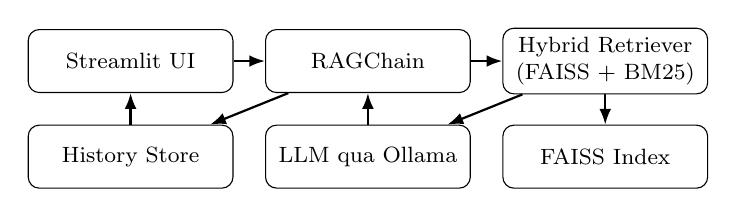
\begin{tikzpicture}[
  node distance=4mm and 4mm,
  box/.style={draw, rounded corners, align=center, minimum height=8mm, minimum width=26mm, font=\footnotesize},
  arr/.style={-{Latex[length=2mm]}, thick}
]
\node[box] (ui) {Streamlit UI};
\node[box, right=of ui] (rag) {RAGChain};
\node[box, right=of rag] (ret) {Hybrid Retriever\\(FAISS + BM25)};
\node[box, below=of rag] (llm) {LLM qua Ollama};
\node[box, left=of llm] (hist) {History Store};
\node[box, right=of llm] (index) {FAISS Index};

\draw[arr] (ui) -- (rag);
\draw[arr] (rag) -- (ret);
\draw[arr] (ret) -- (llm);
\draw[arr] (ret) -- (index);
\draw[arr] (llm) -- (rag);
\draw[arr] (rag) -- (hist);
\draw[arr] (hist) -- (ui);
\end{tikzpicture}
}
\caption{Kiến trúc xử lý của hệ thống hỏi đáp tài liệu}
\label{fig:architecture}
\end{figure}

Sơ đồ này cho thấy RAGChain đóng vai trò trung tâm điều phối. Khi nhận câu hỏi, hệ thống truy xuất ngữ cảnh từ retriever lai, gửi prompt cho LLM, sau đó ghi kết quả vào history để hiển thị lại trên giao diện. Luồng này giúp tách rõ trách nhiệm của từng module và thuận tiện cho bảo trì.

\subsection{Nhật ký triển khai theo commit}
Dựa trên lịch sử commit gần nhất của dự án, tiến độ phát triển có thể tóm tắt theo các mốc chính như sau:
\begin{itemize}
\item Khởi tạo cấu trúc thư mục và bộ thư viện nền.
\item Bổ sung xử lý tài liệu và RAG cơ bản.
\item Chuyển từ vector hóa đơn giản sang \path{FAISS.from_documents()} để giữ metadata.
\item Tích hợp frontend Streamlit và hoàn thiện luồng người dùng.
\item Thêm tính năng lưu history, mở rộng nạp nhiều tài liệu và bổ sung CoRAG.
\end{itemize}
Các mốc trên tương ứng với các commit tiêu biểu: 1e2a7d4, 93d855f, 02a282e, 17b7283, cde5974, 395ec98, e012565.

Từ góc nhìn cá nhân (nội dung mô phỏng phù hợp với tiến độ repo), nhóm tự đánh giá đã học được các điểm sau:
\begin{itemize}
\item Cách tổ chức một ứng dụng AI thành nhiều lớp tách biệt: xử lý dữ liệu, truy xuất, sinh câu trả lời và giao diện.
\item Cách đánh đổi giữa độ chính xác và tốc độ khi chuyển từ RAG sang CoRAG.
\item Kỹ năng đọc log lỗi, vá lỗi nhanh (ví dụ lỗi thiếu thuộc tính, cấu hình môi trường PowerShell, cảnh báo model/caching).
\item Kỹ năng trình bày kết quả có nguồn trích dẫn để tăng tính kiểm chứng cho câu trả lời sinh bởi LLM.
\end{itemize}

\subsection{Kịch bản kiểm thử dựa trên lịch sử chat đã lưu}
Hệ thống đã được kiểm thử lặp lại trên nhiều truy vấn thật trong file history của project. Một số truy vấn tiêu biểu gồm: ``Nội dung tài liệu?'', ``file này nói về gì'', ``các file đã được index nói về gì'' và ``file nào nói về AI''. Kết quả cho thấy luồng RAG thường trả lời nhanh hơn CoRAG trong các câu hỏi tổng hợp ngắn, trong khi CoRAG có xu hướng trả lời đầy đủ hơn khi câu hỏi gồm nhiều ý.

Từ lịch sử test, độ trễ quan sát được nằm trong khoảng khá rộng (xấp xỉ hơn 100 giây đến hơn 230 giây tùy truy vấn, dữ liệu và chiến lược suy luận). Điều này phù hợp với nhận định ở Hình~\ref{fig:relative-cost}: bước sinh câu trả lời của mô hình là nút thắt chính, còn CoRAG tốn thêm thời gian do bước tách câu hỏi và tổng hợp nhiều context.

\subsection{Sơ đồ giải thuật cho một lượt hỏi đáp}
Để thể hiện rõ thành phần ``sơ đồ giải thuật'', Hình~\ref{fig:algorithm-flow} mô tả luồng xử lý của một truy vấn từ lúc nhập câu hỏi đến khi trả kết quả cho người dùng.

\begin{figure}[H]
\centering
\begin{tikzpicture}[
  node distance=5mm,
  proc/.style={rectangle, draw, rounded corners, align=center, text width=0.54\columnwidth, minimum height=7mm, font=\footnotesize},
  dec/.style={diamond, draw, aspect=2.0, align=center, text width=0.30\columnwidth, inner ysep=1pt, font=\footnotesize},
  outbox/.style={rectangle, draw, rounded corners, align=center, text width=0.30\columnwidth, minimum height=7mm, font=\footnotesize},
  line/.style={-{Latex[length=2mm]}, thick}
]
\node[proc] (q) {Nhận câu hỏi};
\node[dec, below=of q] (empty) {Câu hỏi rỗng?};
\node[proc, below=of empty] (retr) {Hybrid retrieve + filter};
\node[dec, below=of retr] (nodoc) {Có tài liệu phù hợp?};
\node[proc, below=of nodoc] (ctx) {Format context + gọi LLM};
\node[proc, below=of ctx] (save) {Lưu history và trả đáp án};
\node[outbox, left=9mm of empty] (ret0) {Trả về thông báo rỗng};
\node[outbox, left=9mm of nodoc] (nf) {Trả về ``không tìm thấy''};

\draw[line] (q) -- (empty);
\draw[line] (empty) -- node[left] {Không} (retr);
\draw[line] (empty.west) -- node[above] {Có} (ret0.east);
\draw[line] (retr) -- (nodoc);
\draw[line] (nodoc) -- node[left] {Có} (ctx);
\draw[line] (nodoc.west) -- node[above] {Không} (nf.east);
\draw[line] (ctx) -- (save);
\end{tikzpicture}
\caption{Sơ đồ giải thuật của một phiên truy vấn}
\label{fig:algorithm-flow}
\end{figure}

Sơ đồ trên nhấn mạnh hai nhánh an toàn: nhánh xử lý câu hỏi rỗng và nhánh không có tài liệu phù hợp. Việc tách các nhánh này giúp hệ thống phản hồi ổn định, hạn chế trường hợp LLM sinh nội dung không có cơ sở.

\begin{table}[H]
\renewcommand{\arraystretch}{1.2}
\caption{Ví dụ các ca kiểm thử ghi nhận trong lịch sử}
\label{tab:test-history}
\centering
\footnotesize
\setlength{\tabcolsep}{3pt}
\begin{tabular}{|L{0.27\columnwidth}|L{0.12\columnwidth}|L{0.13\columnwidth}|L{0.34\columnwidth}|}
\hline
Truy vấn & Chế độ & Độ trễ (s) & Ghi nhận \\
\hline
Nội dung tài liệu? & RAG & 109.59 & Trả lời ngắn gọn, có nguồn \\
\hline
Nội dung tài liệu? & CoRAG & 184.52 & Chi tiết hơn, có sub-question \\
\hline
các file đã được index nói về gì & RAG & 233.74 & Tổng hợp được nhiều tài liệu \\
\hline
các file đã được index nói về gì & CoRAG & 234.41 & Đầy đủ hơn nhưng chậm \\
\hline
file nào nói về AI & RAG & -- & Trả về ``không tìm thấy'' đúng ngữ cảnh \\
\hline
\end{tabular}
\end{table}

Bảng~\ref{tab:test-history} cho thấy hệ thống đã có hành vi ổn định theo kỳ vọng: khi không có bằng chứng trong context, mô hình trả lời từ chối thay vì bịa thông tin. Đây là tiêu chí quan trọng đối với các ứng dụng hỏi đáp tài liệu trong môi trường học thuật.

\section{Kết luận}
Qua dự án này, nhóm đã nắm được quy trình xây dựng một hệ thống hỏi đáp tài liệu hoàn chỉnh từ khâu tiền xử lý, tạo embedding, lập chỉ mục, truy xuất cho đến sinh ngôn ngữ tự nhiên. Quan trọng hơn, nhóm hiểu rõ sự khác nhau giữa RAG và CoRAG: RAG phù hợp với phản hồi nhanh, còn CoRAG phù hợp với câu hỏi phức tạp cần phân tách nhiều lớp thông tin.

Về mặt kỹ thuật, dự án cũng cho thấy vai trò của việc tổ chức mã theo module. Khi giao diện, API, truy xuất và sinh câu trả lời được tách riêng, việc chỉnh sửa hoặc tối ưu từng phần trở nên dễ hơn nhiều. Trong quá trình hoàn thiện hệ thống, nhóm cũng nhận ra rằng hiệu năng không chỉ phụ thuộc vào mô hình lớn hay nhỏ, mà còn nằm ở cách lọc context, số lượng chunk truy xuất và cách viết prompt.

Hạn chế hiện tại của hệ thống là vẫn phụ thuộc khá nhiều vào chất lượng tài liệu đầu vào và hiệu năng của mô hình chạy cục bộ. Với các bộ tài liệu rất lớn hoặc câu hỏi đòi hỏi suy luận sâu, thời gian phản hồi vẫn có thể tăng đáng kể. Đây là hướng cần tiếp tục tối ưu ở các phiên bản sau.

\section{Hướng phát triển (công việc tháng tới)}
Trong thời gian tới, nhóm dự kiến phát triển hệ thống theo ba hướng chính. Thứ nhất là cải thiện tốc độ bằng cách cache kết quả truy xuất, giảm số chunk cần gửi vào LLM và tinh chỉnh chiến lược chọn tài liệu. Thứ hai là tăng chất lượng trả lời bằng cách bổ sung cơ chế đánh giá tự động, ví dụ chấm mức liên quan giữa câu trả lời và nguồn tài liệu. Thứ ba là hoàn thiện giao diện và tính năng quản trị, chẳng hạn thêm phân loại tài liệu theo loại file, lọc theo thời gian upload và xuất lịch sử hỏi đáp ra file.

Ngoài ra, nhóm muốn thử nghiệm thêm các mô hình embedding và LLM khác nhau để so sánh giữa tốc độ và chất lượng. Nếu có điều kiện phần cứng tốt hơn, hệ thống cũng có thể được mở rộng sang chạy GPU hoặc triển khai dưới dạng dịch vụ nội bộ cho nhiều người dùng cùng truy cập.

\section{Tài liệu tham khảo}
\begin{thebibliography}{9}

\bibitem{rag}
P. Lewis et al., ``Retrieval-Augmented Generation for Knowledge-Intensive NLP Tasks,'' \emph{NeurIPS}, 2020. \url{https://arxiv.org/abs/2005.11401}

\bibitem{faiss}
Meta AI, \emph{FAISS: Facebook AI Similarity Search}. \url{https://github.com/facebookresearch/faiss}

\bibitem{streamlit}
Streamlit, \emph{Streamlit Documentation}. \url{https://docs.streamlit.io/}

\bibitem{fastapi}
FastAPI, \emph{FastAPI Documentation}. \url{https://fastapi.tiangolo.com/}

\bibitem{ollama}
Ollama, \emph{Ollama Documentation}. \url{https://ollama.com/}

\bibitem{sentence-transformers}
Sentence-Transformers, \emph{Multilingual MPNet sentence embeddings}. \url{https://www.sbert.net/}

\bibitem{bm25}
S. Robertson and H. Zaragoza, ``The Probabilistic Relevance Framework: BM25 and Beyond,'' \emph{Foundations and Trends in Information Retrieval}, 2009.

\end{thebibliography}

\end{document}
